\chapter{Methodology}
\label{ch:methodology}
This chapter enumerates and describes all the technologies, frameworks, and tools utilized in the development of the volunteer computing platform, along with the reasoning for their selection. Each section provides a detailed explanation of these components, establishing a foundation for the following chapter, \ref{ch:implementation} Implementation.

\section{WebAssembly}
\label{sec:methodology:wasm}
WebAssembly is a key technology in this proposed system, offering several advantages for distributed computing. It provides near-native performance, platform independence, and potential multi-threading capabilities. WebAssembly allows to compile code written in languages such as C, C++, and Rust to a binary format that can be executed in web browsers, enabling efficient computation on diverse client devices.
\subsection{emscriptren for C and C++}
\label{subsec:methodology:wasm:cpp}
\subsection{Go}
\label{subsec:methodology:wasm:go}
\subsection{Pyodie for Python}
\label{subsec:methodology:wasm:python}

\section{WebSokets}
\label{sec:methodology:websokets}
WebSockets play a crucial role in this system's communication infrastructure. Unlike traditional HTTP requests, WebSockets enable faster, bidirectional communication between clients and servers. This real-time capability is essential for efficient task distribution, progress monitoring, and result collection in the distributed computing platform.

\section{WebWorker}
\label{sec:methodology:webworker}
Web Workers are employed to enhance the performance and responsiveness of client-side computations. By executing computationally intensive tasks in separate threads, Web Workers prevent blocking the main thread responsible for the user interface and other critical browser functions. This approach allows our system to utilize client resources more effectively while maintaining a smooth user experience.

\section{Frameworks}
\label{sec:methodology:frameworks}
This section introduces the frameworks selected for the development of the web application. The following criteria were used to guide the selection of a suitable framework for the backend as well as the frontend:
\begin{itemize}
    \item The framework is well-tested and provides a stable \ac{LTS} version.
    \item The framework is popular among web developers.
    \item I am familiar with the programming language.
\end{itemize}

\subsection{Backend}
\label{subsec:methodology:frameworks:backend}
It was crucial for the backend framework to be popular among web developers. Working with a popular framework improves the development process by ensuring the availability of extensive educational and support resources online. Additionally, a widely used framework increases the likelihood that the platform can be maintained or further extended by other programmers.
\begin{figure}[htbp]
 \centering
 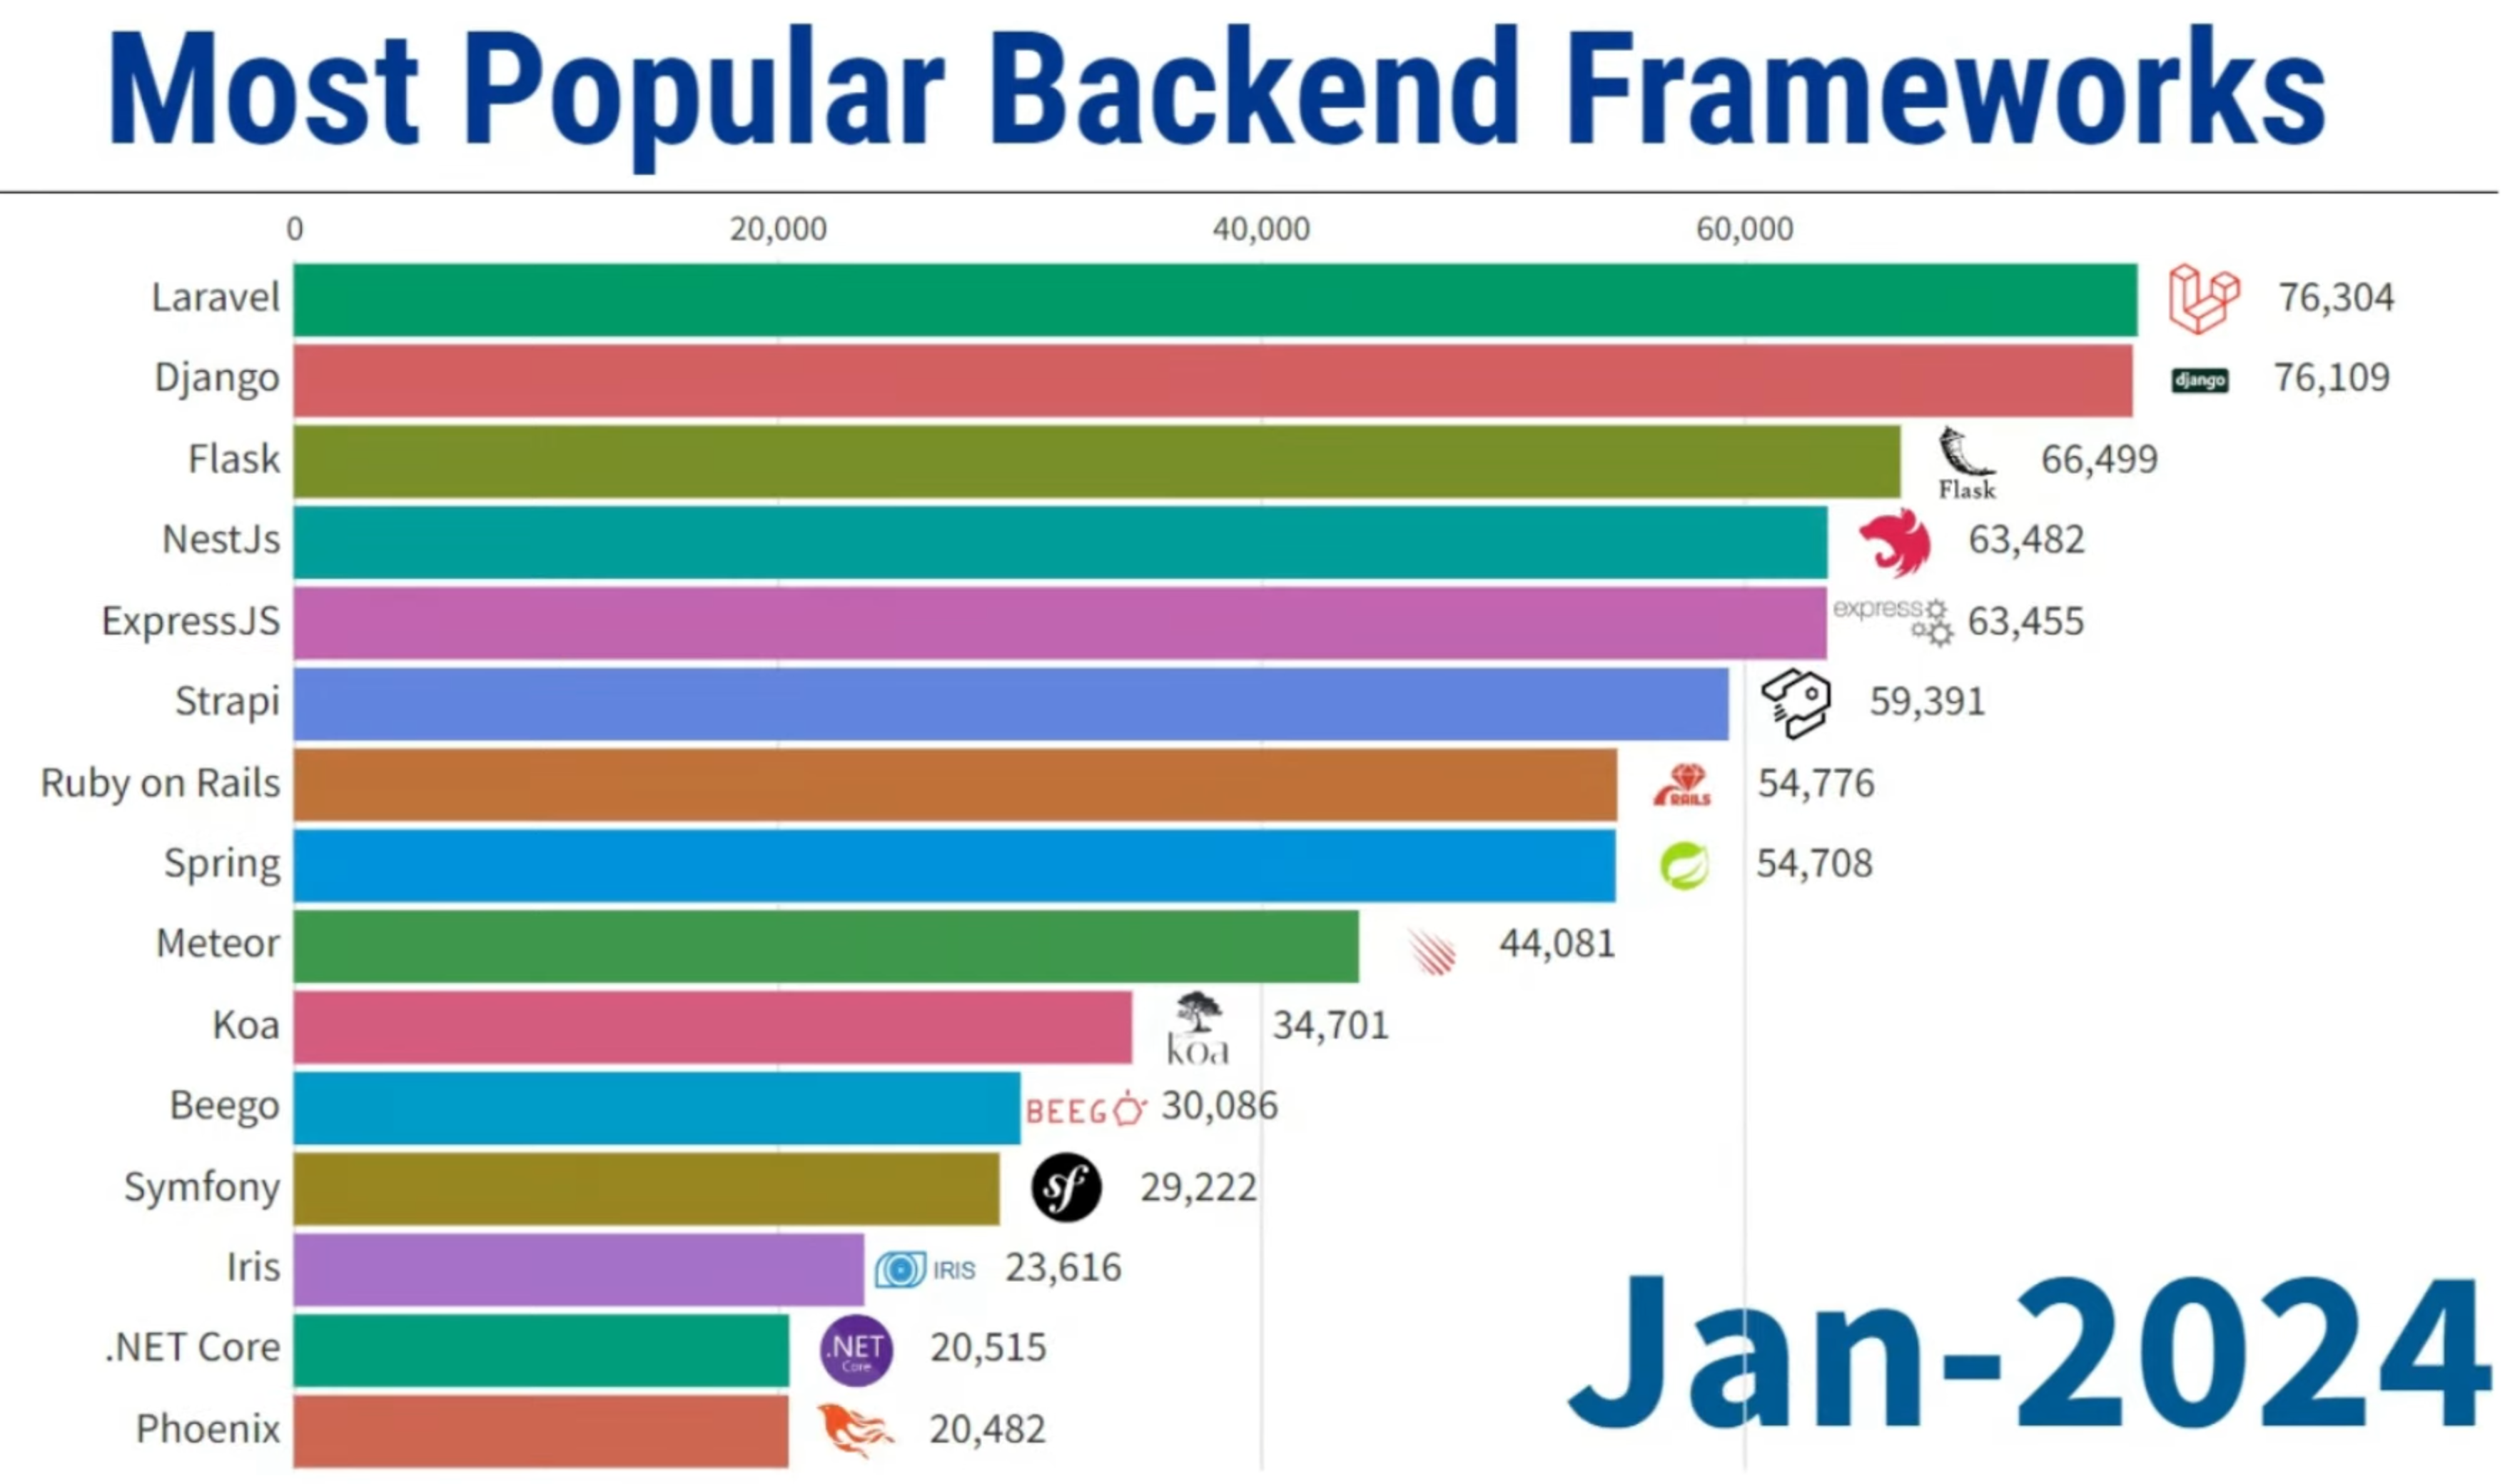
\includegraphics[width=0.95\textwidth]{gfx/figures/Popular_BE.png}
 \caption{Most Popular Backend Frameworks (Jan 2024) by GitHub Stars \cite{backend:popularity}}
 \label{fig:methodology:popularBE}
\end{figure}
The 15 most popular backend frameworks of January 2024 are displayed in figure \ref{fig:methodology:popularBE}. The popularity for each framework of this list is calculated by the number of GitHub Stars from repositories listed in a GitHub Archive \cite{backend:popularity}. The selection options of the backend framework where based on this popularity list. 
\begin{figure}[htbp]
  \myfloatalign
  \subfloat[Requests/Second (2024-06-25) \cite{backend:benchmark1}]{
     \label{fig:methodology:benchmark1BE}
     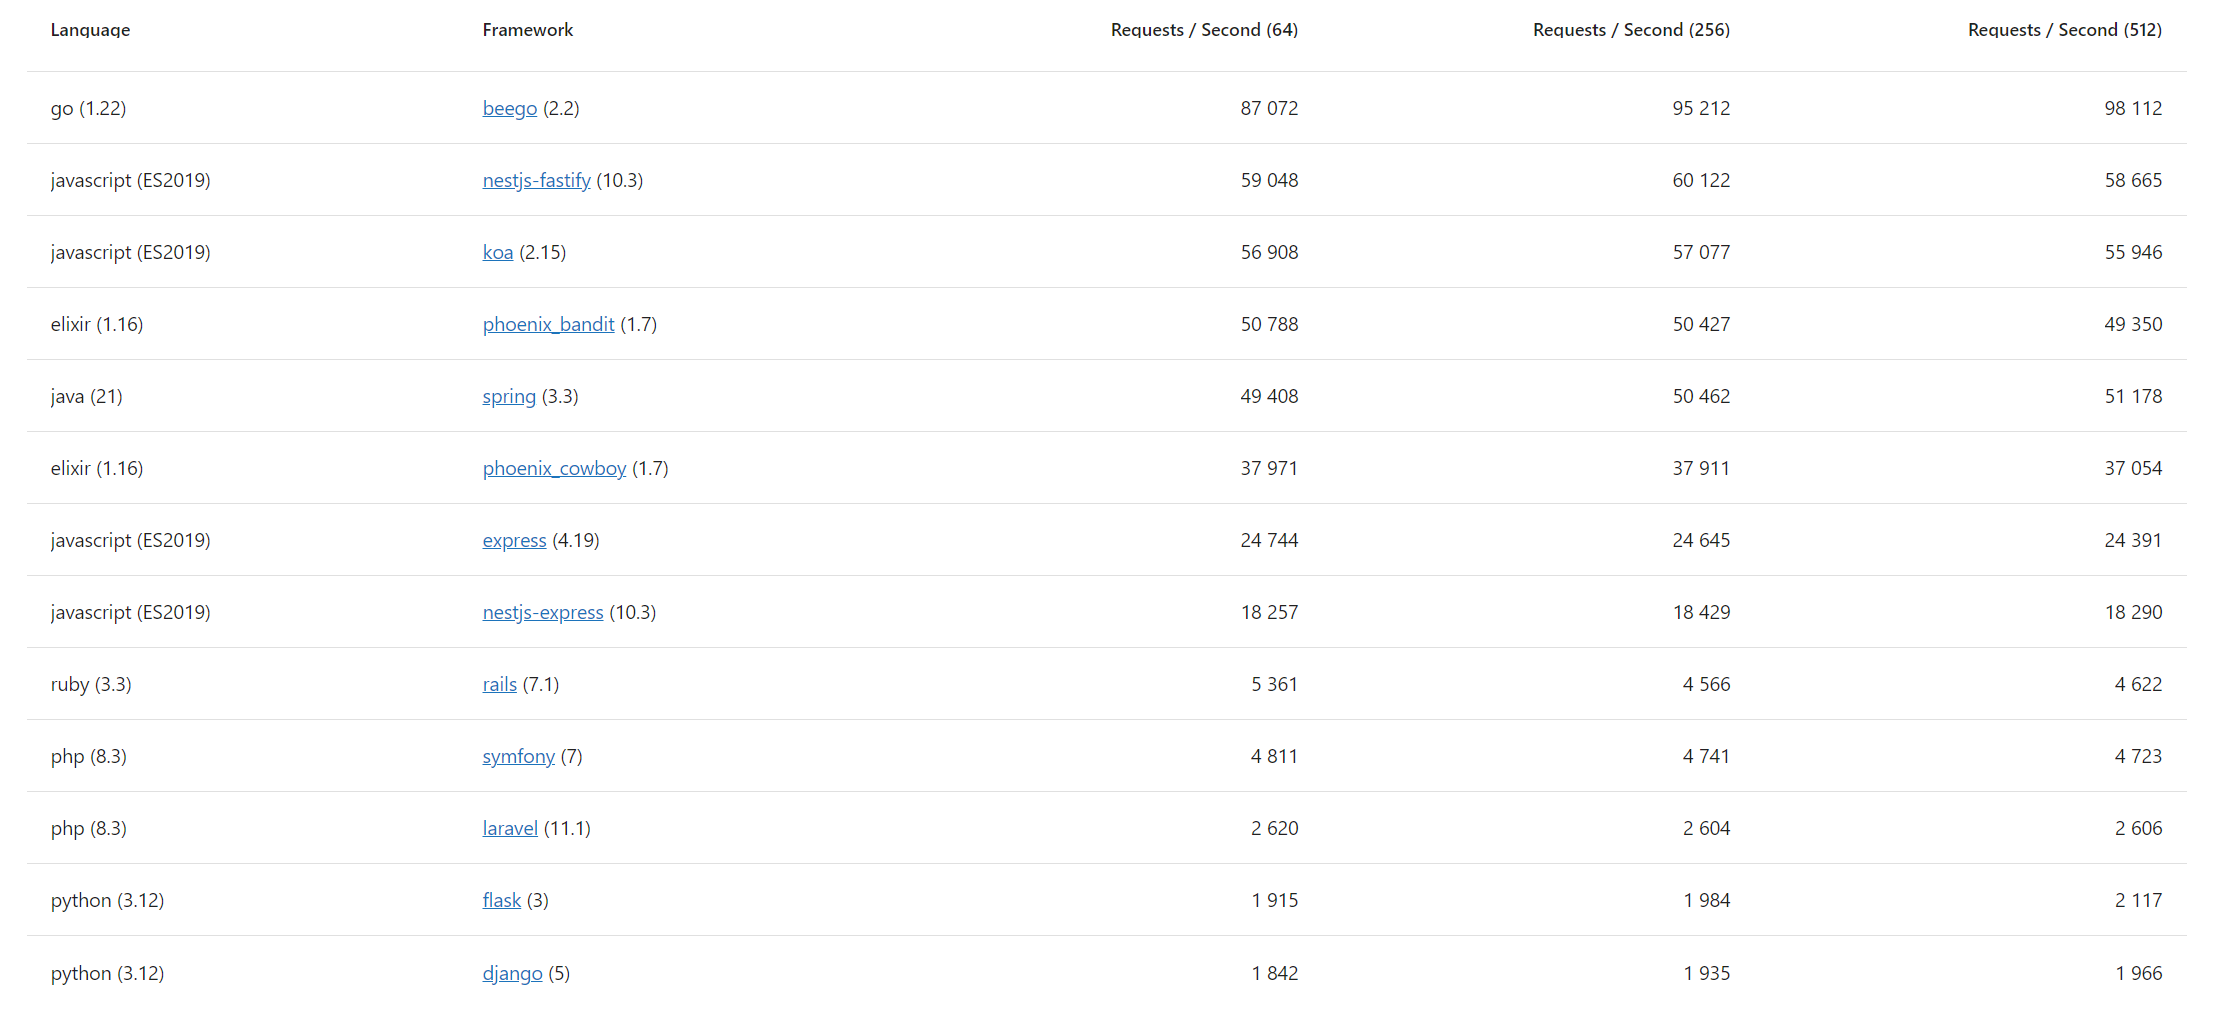
\includegraphics[width=.95\linewidth]{gfx/figures/Benchmark1_BE.png}
   } \\
   \subfloat[Best fortunes responses per second (2023-10-17) \cite{backend:benchmark2}]{
     \label{fig:methodology:benchmark2BE}
     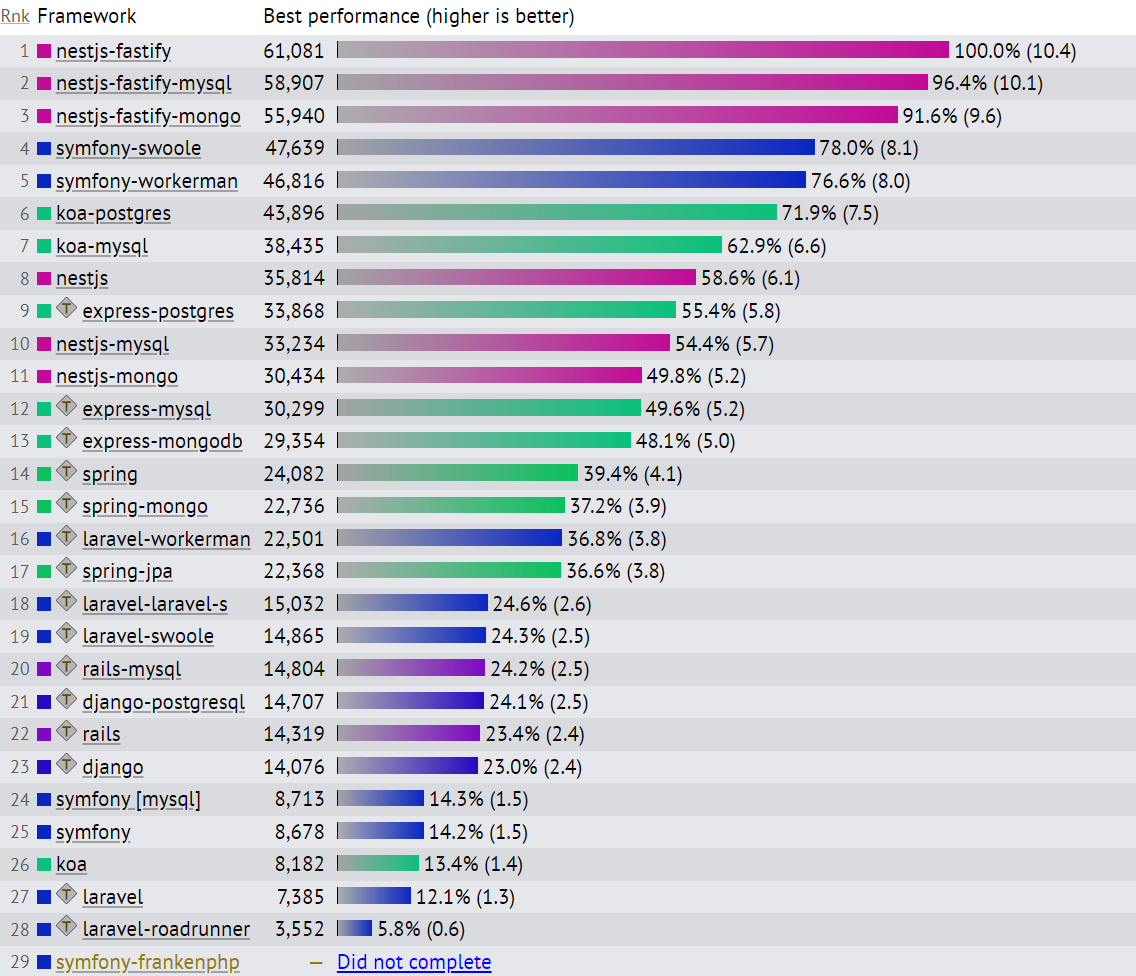
\includegraphics[width=.95\linewidth]{gfx/figures/Benchmark2_BE.png}
   }
   \caption{Most Popular Backend Frameworks from Figure \ref{fig:methodology:popularBE} ranked by Performance.}
   \label{fig:methodology:benchmarkBE}
\end{figure}
In addition to the previously stated criteria, the selected backend framework needed to meet specific performance requirements. It was essential for the framework to efficiently handle multiple connected clients with minimal latency. Furthermore, the framework's internal computation speed was critical, particularly for preparing input arguments for each task and managing task scheduling across all clients. The goal was to reduce overhead as much as possible to ensure high performance.

To identify a high-performance framework, the most popular backend frameworks listed in Figure \ref{fig:methodology:popularBE} were compared using two different benchmarks. The results of these benchmarks are presented in Figure \ref{fig:methodology:benchmarkBE}, where the frameworks are ranked from top to bottom based on their performance in both benchmarks. It is important to note that some frameworks from the list in Figure \ref{fig:methodology:popularBE} could not be found in these specific benchmarks. Both benchmark sources simulated numerous clients sending requests to each backend and measuring the number of successful responses per second in order to determine the performance \cite{backend:benchmark1, backend:benchmark2}.

Finally, NestJS with Fastify was selected as the backend framework. It performed exceptionally well in both benchmarks shown in Figure \ref{fig:methodology:benchmarkBE} and is also a popular choice among developers.

\subsection{Frontend}
\label{subsec:methodology:frameworks:frontend}
Why is NextJs a good choise?

\section{Entities}
\label{sec:methodology:entities}
To define the nomenvclature later in the Thesis and the structure of the Project
\subsection{Job}
\label{subsec:methodology:entities:job}
..
\subsection{Task}
\label{subsec:methodology:entities:task}
..
\subsubsection{Batch}
\label{ssubsec:methodology:entities:task:batch}
What is a batch of Tasks?
\subsection{Client and User Types}
\label{subsec:methodology:entities:client}
..
\subsubsection{User}
\label{ssubsec:methodology:entities:client:user}
worker and donates workpower/Harware executes Software wasm
\subsubsection{Admin}
\label{ssubsec:methodology:entities:client:admin}
administrates Jobs, Distributes Jobs. Does not perform Task execution.
\subsection{Server}
\label{subsec:methodology:entities:task}
Basically the backend

\section{Benchmark: Definition of Job}
\label{sec:methodology:benchmark}
How can i benchmark the platform? What problem / code is used to benchmark? Which hardware is used for the benchmark?